\documentclass{article}
\usepackage[english]{babel}
\usepackage{amsmath}
\usepackage[a4paper,scale=0.75]{geometry}
\usepackage{commath}
\usepackage{mathtools}
\usepackage{tensor}
\usepackage[font=footnotesize, labelfont=bf, labelformat=empty]{caption}
\usepackage{subcaption}
\usepackage{booktabs}
\usepackage{multirow}

\begin{document}
\thispagestyle{empty}
\begin{figure}
    \centering
    \begin{subfigure}{0.3\linewidth}
        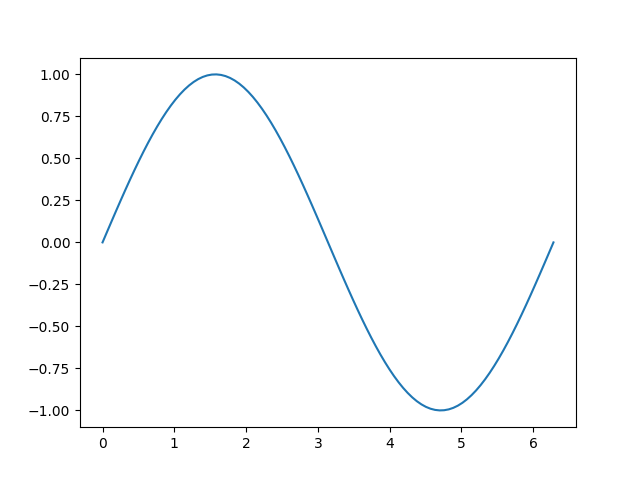
\includegraphics[width=\linewidth]{../figures/sin.png}
        \caption{\(y=\sin x, x\in[0,2\pi]\)}
    \end{subfigure}
    \begin{subfigure}{0.3\linewidth}
        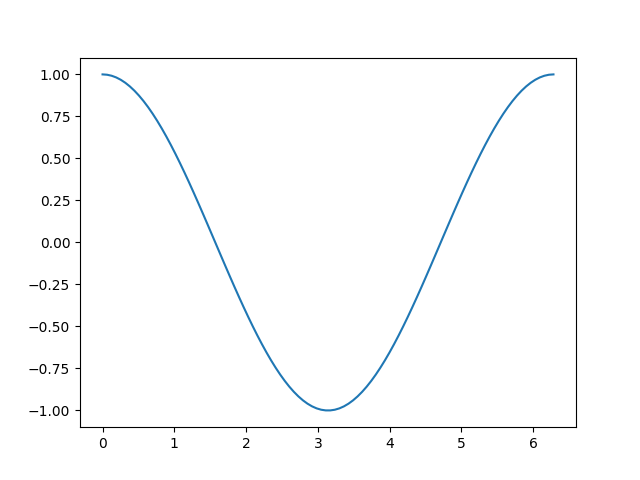
\includegraphics[width=\linewidth]{../figures/cos.png}
        \caption{\(y=\cos x, x\in[0,2\pi]\)}
    \end{subfigure}
    \\
    \begin{subfigure}{0.3\linewidth}
        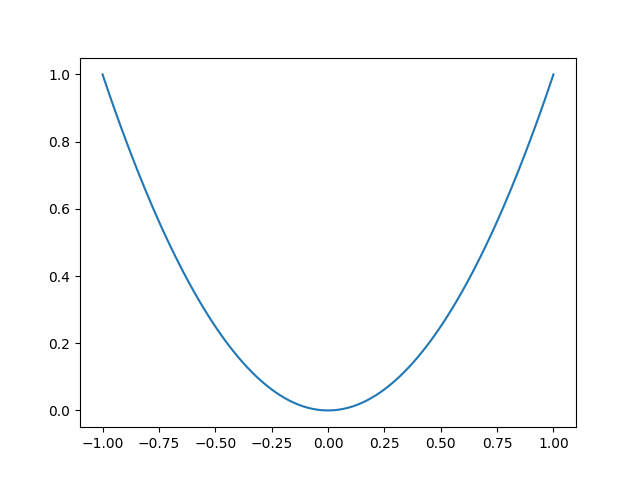
\includegraphics[width=\linewidth]{../figures/square.png}
        \caption{\(y=x^2, x\in[-1,1]\)}
    \end{subfigure}
    \begin{subfigure}{0.3\linewidth}
        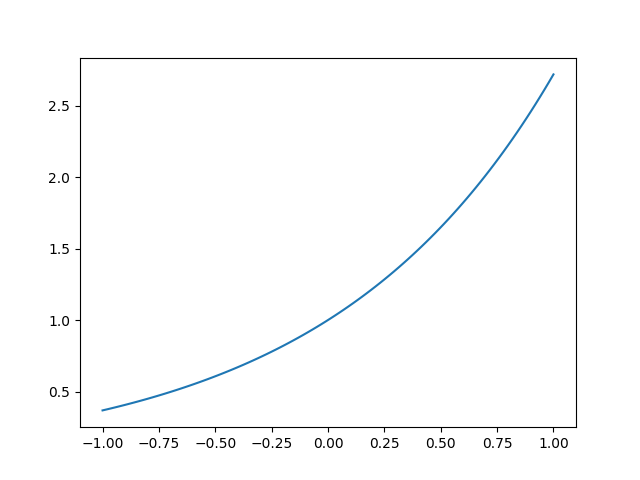
\includegraphics[width=\linewidth]{../figures/exp.png}
        \caption{\(y=\mathrm{e}^x, x\in[-1,1]\)}
    \end{subfigure}
    \caption{\textbf{Figure~\ref{Figure-Subfigures}.} Illustration of subfigures.}\label{Figure-Subfigures}
\end{figure}
\end{document}